\documentclass[tikz,border=6pt]{standalone}
\usepackage{fontspec}
\setmainfont{Noto Sans}
\usepackage{amsmath,amssymb}
\usepackage{tikz}
\usetikzlibrary{arrows.meta,positioning,calc,shapes.geometric}
\definecolor{cudaG}{RGB}{118,185,0}
\definecolor{sadRed}{RGB}{200,60,50}
\definecolor{gsBlue}{RGB}{40,110,190}
\definecolor{bgGray}{RGB}{242,242,242}
\begin{document}
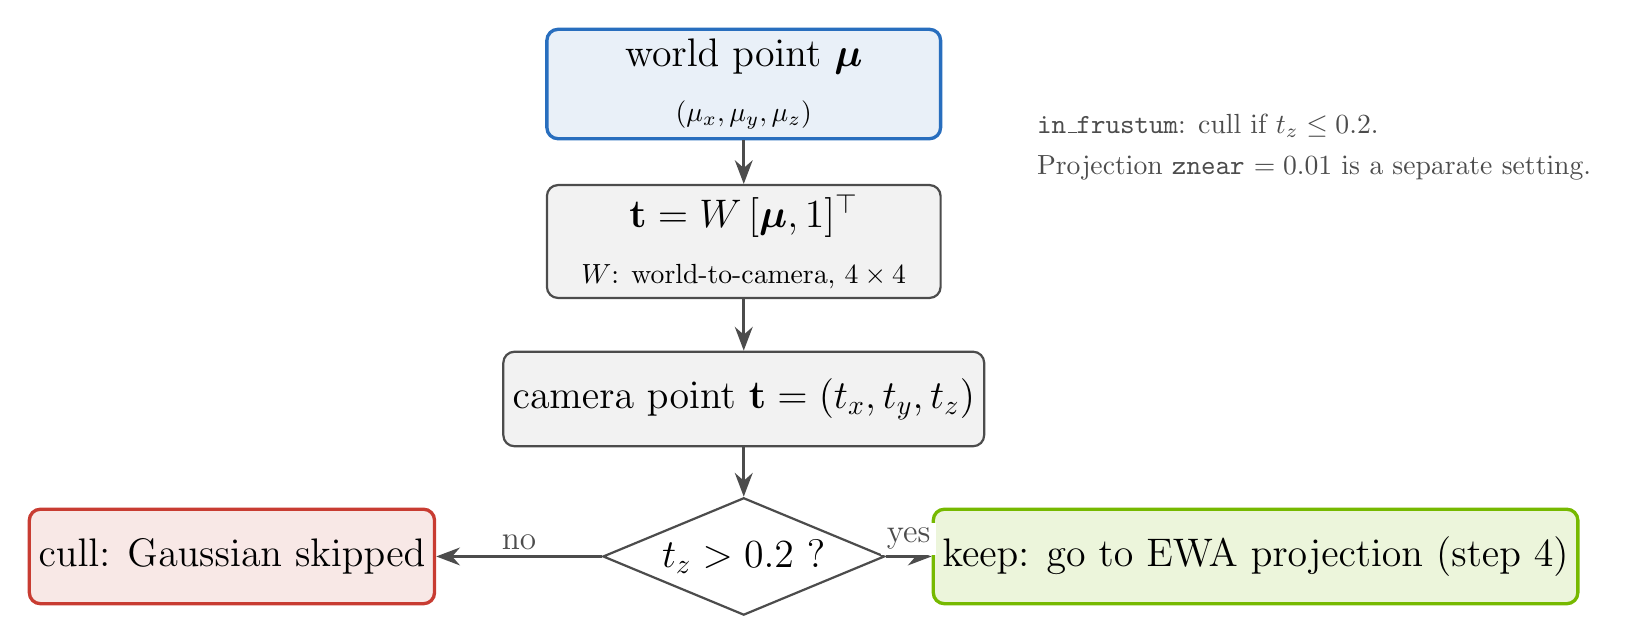
\begin{tikzpicture}[
  inp/.style={draw=gsBlue, very thick, rounded corners, fill=gsBlue!10, minimum width=5cm, minimum height=1.2cm, align=center, font=\Large},
  proc/.style={draw=black!70, thick, rounded corners, fill=bgGray, minimum width=5cm, minimum height=1.2cm, align=center, font=\Large},
  ok/.style={draw=cudaG, very thick, rounded corners, fill=cudaG!14, minimum width=5cm, minimum height=1.2cm, align=center, font=\Large},
  bad/.style={draw=sadRed, very thick, rounded corners, fill=sadRed!12, minimum width=5cm, minimum height=1.2cm, align=center, font=\Large},
  dec/.style={diamond, aspect=2.4, draw=black!70, thick, fill=white, align=center, font=\Large, inner sep=2pt},
  arr/.style={-{Stealth[length=3mm]}, very thick, black!70},
  lab/.style={font=\large, text=black!70, fill=white, inner sep=2pt}
]
  \node[inp] (mu) at (0,6) {world point $\boldsymbol{\mu}$\\[2pt]{\normalsize $(\mu_x,\mu_y,\mu_z)$}};
  \node[proc] (W) at (0,4) {$\mathbf{t}=W\,[\boldsymbol{\mu},1]^{\top}$\\[2pt]{\normalsize $W$: world-to-camera, $4\times4$}};
  \node[proc] (t) at (0,2) {camera point $\mathbf{t}=(t_x,t_y,t_z)$};
  \node[dec] (d) at (0,0) {$t_z > 0.2$ ?};
  \node[ok] (yes) at (6.5,0) {keep: go to EWA projection (step 4)};
  \node[bad] (no) at (-6.5,0) {cull: Gaussian skipped};

  \draw[arr] (mu) -- (W);
  \draw[arr] (W) -- (t);
  \draw[arr] (t) -- (d);
  \draw[arr] (d) -- node[lab,above] {yes} (yes);
  \draw[arr] (d) -- node[lab,above] {no} (no);

  \node[font=\normalsize, text=black!70, align=left, anchor=west] at (3.6,5.2)
    {\texttt{in\_frustum}: cull if $t_z\le 0.2$.\\[3pt]
     Projection \texttt{znear} $=0.01$ is a separate setting.};
\end{tikzpicture}
\end{document}
